%\documentclass{book}
%\begin{document}
\chapter{Definizione del problema}
\setcounter{section}{1}
(replicazione dei dati - introduzione)
\item
\subsection{Cluster di database}
Un cluster \`{e} una raccolta di componenti che garantisce scalabit\`{a} e disponibilit\`{a} distribuendone i costi. Un cluster di database (SQL usa il termine cluster di catalogo) \`{e} una collezione di database gestiti da una singola istanza di un server database in esecuzione. Un'istanza \`{e} la raccolta di memoria e processi che interagiscono con un database, cio\`{e} l'insieme di file fisici che effettivamente memorizzano i dati.\cite{etichetta1} A tal fine, \`{e} possibile creare un cluster di database per applicazioni enterprise high-end, memorizzando e elaborando informazioni sui nodi.\\ L'architettura per un cluster di database \`{e} distinta da come le responsabilit\`{a} dei dati sono condivise tra i nodi di calcolo.

Seguono due dei vantaggi principarli offerti dal clustering, specialmente in un ambiente di database di alto volume:
\begin{itemize}
\item 
\textit{Fault tolerance} (tolleranza di guasti): in caso di guasto del singolo server, il cluster offre un'alternativa, poich\'{e} esiste pi\`{u} di un server o istanza per gli utenti a cui connettersi.
\item
\textit{Load balancing} (bilanciamento del carico): la funzionalit\`{a} di clustering \`{e} generalmente impostata per consentire agli utenti di essere assegnati automaticamente al server con il minor carico.\cite{etichetta1} 
\end{itemize}
Ci sono differenti tipi di architetture clustering che si diversificano da come vengono memorizzati i dati e allocate le risorse.
La prima modalit\`{a} di clustering \`{e} conosciuta come architettura "\textit{shared-nothing}" (SN). \`{E} un'architettura di elaborazione distribuita in cui ogni nodo/server \`{e} totalmente indipendente e autonomo, pertanto nessuno dei nodi condivide memoria o archiviazione del disco. Pi\`{u} generalmente, non esiste un unico punto di contesa nel sistema.\cite{etichetta5} Il partizionamento \`{e} tale che ogni nodo possiede un sottoinsieme dei dati, ovvero ogni nodo ha accesso esclusivo su quel particolare sottoinsieme. 
%((Un esempio di questa forma di clustering potrebbe essere quando un'azienda ha pi\`{u} data centers per un unico sito web. Con molti server in tutto il mondo, nessun singolo server \`{e} un "master"
\cite{etichetta2}))\\

\begin{figure}[htbp]
\centering
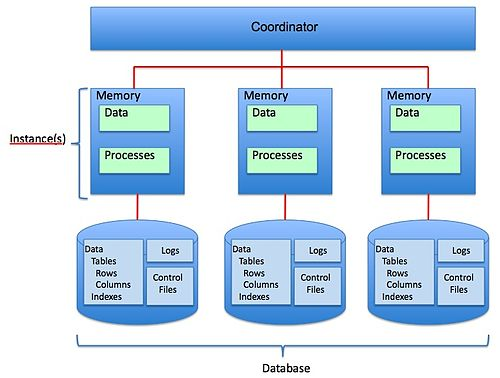
\includegraphics[scale=0.70]{img/Shared_Nothing_Architecture.jpg}\\
\caption{Architecture Shared Nothing \label{figura1.1} \cite{etichetta7}}
\end{figure}

I vantaggi dell'architettura SN rispetto a un'entit\`{a} centrale che controlla la rete (un'architettura basata su controller) riguarda l'eliminazione di qualsiasi singolo punto di guasto, consentendo funzionalit\`{a} di auto-riparazione (\textit{self-healing}) e fornendo un vantaggio nell'offrire aggiornamenti non distruttivi.\cite{etichetta6} 
%\textbf{DA LEGGERE PER BENE ARTICOLO CITATO.}
\textit{Shared-nothing} \`{e} anche noto come "\textit{database sharding}". In generale, un sistema SN divide i suoi dati in vari nodi su database diversi o pu\`{o} richiedere a ciascun nodo di mantenere la propria copia dei dati dell'applicazione utilizzando un qualche tipo di protocollo di coordinamento.\cite{etichetta5}\\


Si oppone a quest'ultima, l'architettura nota come "\textit{shared-disk}" (disco condiviso), in cui tutti i dati vengono memorizzati centralmente in un unico disco e sono accessibili da tutti i nodi di cluster.\cite{etichetta7} In questo tipo di struttura quindi pi\`{u} istanze di database vengono raggruppate in un singolo database sul disco. Nei sistemi di dischi condivisi, i blocchi (o pagine) di dati su disco possono avere un solo proprietario.((
%La propriet\`{a} dei blocchi (o pagine) viene trasferita all'istanza che sta facendo l'aggiornamento. Questo genera traffico di rete e in genere un'infrastruttura dedicata viene implementata tra le istanze di database per far fronte a questo traffico.))
L'architettura \textit{shared-disk} \`{e} un esempio di \textit{Synchronous multi-master}, ovvero ogni istanza del database pu\`{o} scrivere (cio\`{e} \`{e} un master) in modo sincrono.\cite{etichetta7}
\textbf{DA CHIEDERE E DA CONTROLLARE ULTIME FRASI. GUARDA COMMENTO per il sito}
%https://en.wikibooks.org/wiki/Oracle_and_DB2,_Comparison_and_Compatibility/Database_Scaling/Shared_Architectures}}

\begin{figure}[htbp]
\centering
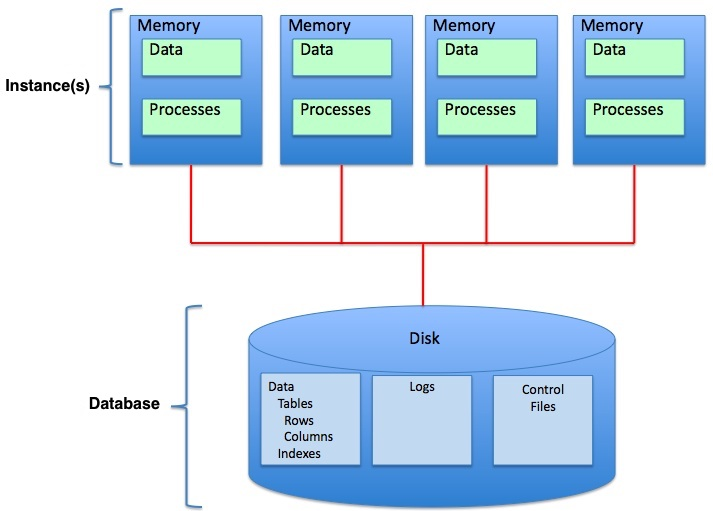
\includegraphics[scale=0.40]{img/Shared_Disk_Architecture.jpg}\\
\caption{Architecture Shared Disk - Shared Everything \label{figura1.2} \cite{etichetta7}}
\end{figure}

In un'architettura SD, grandi reti di computer possono operare su un singolo set di dati senza la necessit\`{a} di replicare o bloccare quel set di dati.\cite{etichetta7}
\textit{Shared disk} ha due vantaggi:
\begin{itemize}
\item
ogni processore ha la propria memoria, 
\item
il bus di memoria non \`{e} un collo di bottiglia (contrariamente all'architettura "\textit{shared-everything}"), 
\item 
il sistema offre un modo semplice per fornire un certo grado di tolleranza agli errori.\\
\end{itemize}
La distinzione tra i due tipi \`{e} diventata confusa di recente con l'introduzione di distribuzione della cache. In questa configurazione, i dati sono ancora gestiti centralmente, ma controllati da un potente "server virtuale" composto da molti server che lavorano insieme come uno.\cite{etichetta2}

\item
\subsection{Rete di pari}
\textit{Peer-to-peer networking} (P\verb"2"P) \`{e} un modello di comunicazione decentralizzato in cui ciascuna parte ha la stessa responsabilit\`{a} per l'elaborazione dei dati e ciascuna parte pu\`{o} avviare una sessione di comunicazione. A differenza del modello\textit{ client/server}, in cui il client effettua una richiesta di servizio e il server soddisfa la richiesta, il modello di rete P\verb"2"P, noto anche come \textit{peer networking}, consente a ciascun nodo di funzionare sia come client che come server.\cite{etichetta13}\\
Quando una rete P\verb"2"P viene stabilita su Internet, \`{e} possibile utilizzare un server centrale per indicizzare i file oppure stabilire una rete distribuita in cui la condivisione dei file viene suddivisa tra tutti gli utenti della rete che memorizzano un determinato file. Le dimensioni della rete e i file disponibili consentono di condividere enormi quantit\`{a} di dati.\\ 
Le prime reti P\verb"2"P come Napster utilizzavano il software client e un server centrale, mentre reti successive come Kazaa e BitTorrent eliminavano il server centrale e dividevano i compiti di condivisione tra pi\`{u} nodi per liberare la larghezza di banda.\\


Seguono i vantaggi di una rete \textit{peer-to-peer}:
\begin{itemize}
\item
se un dispositivo collegato interrompe la connessione, il servizio non termina a differenza del modello \textit{client-server},

\item 
\`{e} possibile configurare i computer in gruppi di lavoro \textit{peer-to-peer} per consentire la condivisione di file e altre risorse su tutti i dispositivi. \textit{Peer networking} consente di condividere facilmente i dati in entrambe le direzioni, sia per i \textit{download} sul computer che per gli \textit{upload} dal computer,

\item
su Internet, le reti peer-to-peer gestiscono un volume elevato di traffico di condivisione file distribuendo il carico su pi\`{u} computer. Poich\'{e} non si basano esclusivamente sui server centrali, le reti P\verb"2"P possono scalare meglio e sono pi\`{u} resistenti delle reti \textit{client-server} in caso di guasti o colli di bottiglia del traffico,

\item
Le reti \textit{peer-to-peer} sono relativamente facili da espandere. Con l'aumentare del numero di dispositivi nella rete, aumenta la potenza della rete P\verb"2"P, poich\'{e} ogni computer aggiuntivo \`{e} disponibile per l'elaborazione dei dati.\cite{etichetta14}
\end{itemize}

Le reti \textit{peer-to-peer} sono vulnerabili agli attacchi di sicurezza. Poich\'{e} ogni dispositivo partecipa al traffico di routing attraverso la rete, gli hacker possono facilmente lanciare attacchi \textit{denial of service}.
Il software P\verb"2"P funge da server e client, il che rende le \textit{peer networking} pi\`{u} vulnerabili agli attacchi remoti rispetto alle reti client-server.
I dati corrotti possono essere condivisi su reti P\verb"2"P modificando i file gi\`{a} presenti in rete per introdurre codice dannoso.\cite{etichetta14}

\item
\subsection{Sistemi di ridondanza disco (RAID)}
RAID, acronimo di \textit{redundant array of independent disks}, insieme ridondante di dischi indipendenti (originariamente \textit{redundant array of inexpensive disks}), \`{e} una tecnologia che permette di memorizzare dati su pi\`{u} dischi rigidi in un computer (o collegati ad esso) in modo da garantire una gestione sicura dei dati\cite{etichetta9}. I dispositivi RAID sono convenienti per sistemi che abbiano necessit\`{a} di grandi quantit\`{a} di dati continuamente disponibili. 

%Consente di ottenere quindi determinate caratteristiche di protezione e velocit\`{a} su sistemi "casalinghi" su dischi economici, in contrapposizione a configurazioni riservate per sistemi professionali ben pi\`{u} costosi.
%((Il RAID può essere implementata anche nei PC normali, sono infatti disponibili schede raid a basso costo quando non già presente sulle schede madri più sofisticate, ma è una tecnica tipicamente storicamente impiegata nei server o nelle workstation che richiedano grandi volumi o elevate prestazioni di immagazzinamento di dati, ad esempio per ospitare una base di dati)).\\ 

Il RAID, con modalit\`{a} differenti a seconda del tipo di configurazione, trae vantaggio dai principi di ridondanza dei dati e di parallelismo in modo da ottenere:
\begin{itemize}
\item 
incrementi di prestazioni (in lettura/scrittura);
\item
aumenti nella capacit\`{a} di memorizzazione disponibile;
\item 
miglioramenti nella tolleranza ai guasti, ne segue migliore affidabilit\`{a}\cite{etichetta10}. Il RAID rende il sistema resiliente alla perdita di uno o pi\`{u} hard disk, permettendo di sostituirli senza l'interruzione del servizio.
\end{itemize}

I volumi RAID vengono percepiti dal sistema operativo come una singola unit\`{a}, indipendentemente dal numero di componenti che li costituiscono.

Il RAID funziona mettendo i dati su pi\`{u} dischi e consentendo operazioni di input/output (I/O) di sovrapporsi in modo equilibrato. Poich\'{e} l'utilizzo di pi\`{u} dischi aumenta il tempo medio tra i guasti, memorizzare i dati ridondantemente aumenta la tolleranza agli errori.\\

I dati vengono suddivisi in "\textit{stripes}", ovvero in sezioni di stessa  lunghezza, detta l'unit\`{a} del sezionamento e scritti su differenti dischi. Quando si richiede una lettura di dimensione superiore all'unit\`{a} di sezionamento, diverse implementazioni di diversi sistemi RAID distribuiscono l'operazione su pi\`{u} dischi in parallelo, aumentando le prestazioni. Ad esempio, se abbiamo sezioni da 1 bit e un array di D dischi, le sequenze di dati lunghe almeno D bit sfruttano tutti i dischi. \textbf{preso tutto da wikipedia}

\item
\subsubsection{RAID hardware e software}
Il RAID pu\`{o} essere implementato sia con hardware dedicato che con software specifico.

Nel primo caso si tratta di unit\`{a} di controllo che gestiscono tutto autonomamente, facendo in modo che il sistema operativo veda un disco normale. 
Nel secondo caso, \`{e} il sistema operativo che associa i dischi e li gestisce usando una forma di ridondanza attraverso un normale controller (ATA, SCSI, Fibre Channel o altro).

Le unit\`{a} di controllo RAID sono pi\`{u} costose di quelle normali; tuttavia, se non si creano altri tipi di problemi, hanno il vantaggio di non creare difficolt\`{a} al sistema operativo.
%http://www.webalice.it/climberjak/linux_informatica/gestione_dei_dischi_in_modo_ridondante.htm

\item
\subsubsection{Controllore RAID}
Un controller RAID \`{e} un dispositivo hardware o un programma software utilizzato per gestire unit\`{a} disco fisso (HDD) o unit\`{a} SSD (\textit{Solid State Drive}, SSD) in un computer o un array di archiviazione in modo da funzionare come unit\`{a} logica.

Un controller offre un livello di astrazione tra un sistema operativo e le unit\`{a} fisiche. Un controller RAID presenta gruppi a applicazioni e sistemi operativi come unit\`{a} logiche per le quali \`{e} possibile definire schemi di protezione dei dati. Poich\'{e} il controller ha la possibilit\`{a} di accedere a pi\`{u} copie di dati su pi\`{u} dispositivi fisici, ha la capacit\`{a} di migliorare le prestazioni e proteggere i dati in caso di crash di sistema.

Nel RAID hardware, un controller fisico viene utilizzato per gestire l'array RAID. Il controller pu\`{o} assumere la forma di una scheda PCI o PCI Express (PCIe), progettata per supportare un formato di unit\`{a} specifico come SATA o SCSI (alcuni controller RAID possono anche essere integrati con la scheda madre.) 

Un controller RAID pu\`{o} anche essere solo software, utilizzando le risorse hardware del sistema host. Il RAID basata su software generalmente fornisce funzionalit\`{a} simili a RAID \textit{hardware-based}, ma la sua prestazione \`{e} tipicamente inferiore a quella delle versioni hardware.\cite{etichetta12}

\item
\subsubsection{Livelli RAID}
La caratteristica fondamentale che identifica una configurazione RAID \`{e}, come citato in precedenza, l'array, che rappresenta il tipo di collegamento logico che c'\`{e} tra i vari dischi.
Con tale criterio viene determinato il livello RAID, ovvero la configurazione della tipologia di RAID  e stabilito il numero minimo di hard disk che sono necessari per attivarlo. A seconda del livello RAID sono implementate diverse caratteristiche operative per ottenere maggiori prestazioni o una maggiore sicurezza dei propri dati oppure entrambe le condizioni.\\
Si distinguono sei livelli, da \verb"0" a \verb"5".
Questo sistema numerato consente di differenziare le versioni e di scegliere come diffondere i dati attraverso l'array ed \`{e} stato suddiviso in tre categorie: livelli RAID standard, nidificati e non standard\cite{etichetta9} (segue la descrizione dei livelli standard e qualche nidificato).

\paragraph{Livelli RAID Standard}
\begin{itemize}
\begin{figure}[htbp]
\item 
\verb"RAID 0": livello privo di ridondanza. Si occupa di unire due o pi\`{u} dischi, all'interno dei quali i dati vengono suddivisi equamente (tramite striping o sezionamento), in modo da bilanciare anche il carico di operazioni di lettura e scrittura che li riguardano. Livello che consente di realizzare un disco virtuale di grandi dimensioni, pi\`{u} efficiente, ma la rottura di uno dei dischi porta alla perdita di tutti i dati. 

\verb"RAID 0" \`{e} noto anche con il nome di \textit{block striping}.\textbf{bibliografia commentata}\\
%http://www.webalice.it/climberjak/linux_informatica/gestione_dei_dischi_in_modo_ridondante.htm

\centering
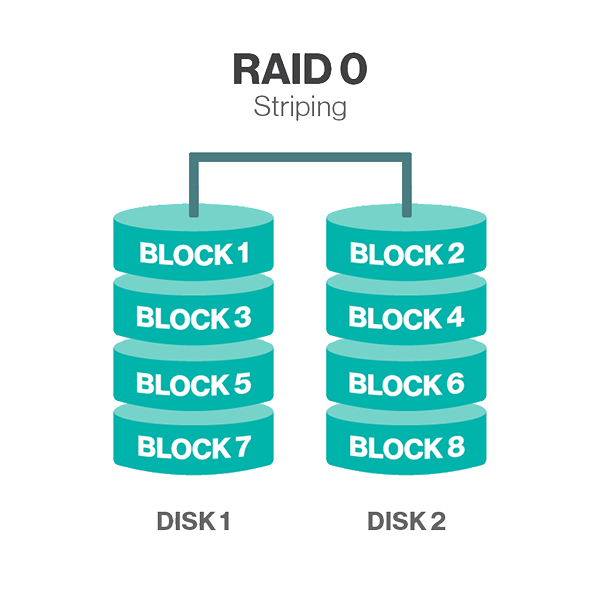
\includegraphics[scale=0.40]{img/raid00.png}\\
\caption{Sezionamento senza ridondanza - Questa configurazione ha sezionamento, ma nessuna ridondanza dei dati. Offre le migliori prestazioni, ma nessuna tolleranza agli errori.\label{figura1.3}\cite{etichetta9}}
\end{figure}

\begin{figure}[htbp]
\item 
\verb"RAID 1": livello che si occupa di unire assieme due o pi\`{u} dischi riproducendo fedelmente gli stessi dati. Questa configurazione mantiene quindi almeno una copia esatta di tutti i dati, detta "\textit{mirror}". In questo caso, la rottura di un disco non pregiudica l'utilizzo dei dati che sono disponibili nel disco o nei dischi rimanenti. Pi\`{u} precisamente, l'affidabilit\`{a} aumenta linearmente al numero di dischi presenti: un sistema con \verb"N" dischi \`{e} in grado di resistere alla rottura di \verb"N-1" componenti.\\ La lettura delle prestazioni \`{e} migliorata poich\'{e} entrambi i dischi possono essere letti contemporaneamente. La scrittura delle prestazioni \`{e} la stessa di quella per il singolo disco.\cite{etichetta9} 

\verb"RAID 1" \`{e} conosciuto anche come \textit{disk mirroring}.\\
%http://www.webalice.it/climberjak/linux_informatica/gestione_dei_dischi_in_modo_ridondante.htm

%DA WIKIPEDIA
%A livello prestazionale, il sistema RAID 1 aumenta tipicamente i risultati per le operazioni di lettura, perché molte implementazioni sono in grado di effettuare diverse operazioni in parallelo: mentre la lettura di un blocco è ancora in corso su un disco, cioè, possono effettuarne un'altra su un disco diverso. In ogni caso, la velocità di lettura raggiunge quella del disco più veloce in presenza di dispositivi di memorizzazione con prestazioni diverse: una singola operazione di lettura è richiesta inizialmente e contemporaneamente su tutti i dischi, ma si conclude nel momento della prima risposta ricevuta. Viceversa, la velocità di scrittura scende a quella del disco più lento, perché questo tipo di azione richiede il compimento della replica della stessa operazione su ogni disco dell'insieme.
\centering
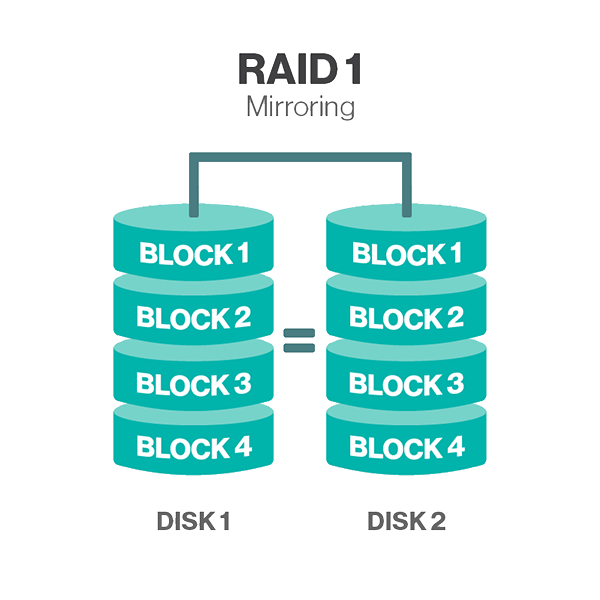
\includegraphics[scale=0.40]{img/raid11.png}\\
\caption{Replicazione - Questa configurazione \`{e} costituita da almeno due unit\`{a} che duplicano la memorizzazione dei dati. Non c'\`{e} sezionamento.\label{figura1.4} \cite{etichetta9}}
\end{figure}

\begin{figure}[htbp]
\item
\verb"RAID 2": livello che divide i dati al livello di bit (invece che di blocco) e usa un \textit{codice di Hamming} per la correzione d'errore che permette di correggere errori su singoli bit e di rilevare errori doppi. Questi dischi sono sincronizzati dal controllore, in modo tale che la testina di ciascun disco sia nella stessa posizione in ogni disco.\cite{etichetta10}\\
%Questa configurazione si rivela molto efficiente in ambienti in cui si verificano numerosi errori di lettura o scrittura, ma in ambienti pi\`{u} prestanti, data l'elevata affidabilit\`{a} dei dischi, il \verb"RAID 2" non viene utilizzato.

\centering
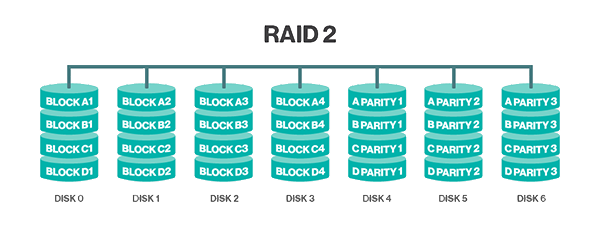
\includegraphics[scale=0.50]{img/raid22.png}\\
\caption{Sezionamento a livello di bit - Questa configurazione ha alcuni dischi che memorizzano le informazioni di errore di verifica e correzione (ECC).\label{figura1.6} \cite{etichetta9}}
\end{figure}

\begin{figure}[htbp]
\item
\verb"RAID 3": livello che si occupa di unire assieme almeno tre o pi\`{u} dischi, all'interno dei quali i dati vengono suddivisi equamente, in modo da bilanciare anche il carico di operazioni di lettura e scrittura che li riguardano. Dedicano uno di questi dischi al contenimento di un sistema di codici di controllo, che permettono di ricostruire i dati nel caso in cui uno degli altri dischi si rompa. Le informazioni ECC vengono utilizzate per rilevare gli errori. Il recupero dei dati viene effettuato calcolando l'esclusiva \verb"OR" (\verb"XOR") delle informazioni registrate sulle altre unit\`{a}.\cite{etichetta9}\\ %Poiché un'operazione di I / O indirizza contemporaneamente tutte le unità, RAID 3 non può sovrapporre I / O. Per questo motivo, RAID 3 è la soluzione ideale per i sistemi a singolo utente con applicazioni di registrazione a lungo termine.

%http://www.webalice.it/climberjak/linux_informatica/gestione_dei_dischi_in_modo_ridondante.htm
\centering
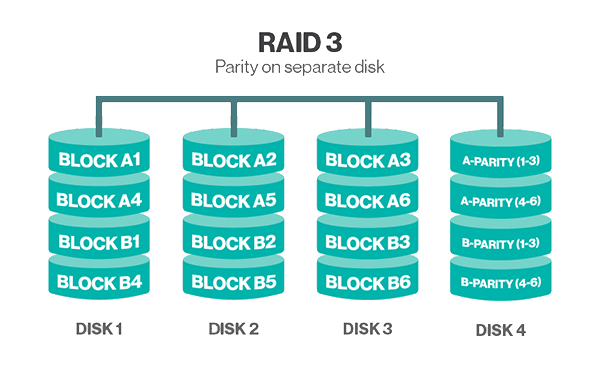
\includegraphics[scale=0.40]{img/raid33.png}\\
\caption{Sezionamento a livello di byte con disco di parit\`{a} - Questa configurazione utilizza la rigatura e dedica un'unit\`{a} a memorizzare informazioni di parit\`{a}.\label{figura1.7} \cite{etichetta9}}
\end{figure}

\begin{figure}[htbp]
\item
\verb"RAID 4": livello simile al livello tre, con la differenza che i dati vengono distribuiti in modo pi\`{u} efficiente tra i dischi, ma rimane compito di un disco separato il sistema di codici di controllo che permette la ricostruzione dei dati, chiamati "blocchi di parit\`{a}".\\
Questo livello utilizza grandi sezionamenti, il che significa che \`{e} possibile leggere i record da un'unica unit\`{a}.\cite{etichetta9}\\

%http://www.webalice.it/climberjak/linux_informatica/gestione_dei_dischi_in_modo_ridondante.htm
\centering
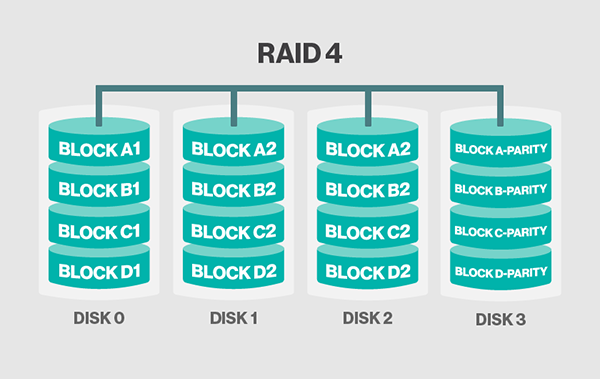
\includegraphics[scale=0.40]{img/raid44.png}\\
\caption{Sezionamento a livello di blocco con disco di parit\`{a}\label{figura1.8} \cite{etichetta9}}
\end{figure}

\begin{figure}[htbp]
\item
\verb"RAID 5": livello basato su livello di blocco con parit\`{a} che risiedono su ciascuna unit\`{a}. L'architettura dell'array consente alle operazioni di lettura e scrittura di coprire pi\`{u} unit\`{a}. Ci\`{o} determina prestazioni migliori di quelle di un'unit\`{a} singola, ma non altrettanto elevata di quella di un array \verb"RAID 0".\cite{etichetta9}\\
%livello equivalente al livello quattro, dove per\`{o} le informazioni che servono per la ricostruzione dei dati sono distribuite tra i dischi, senza essere cos\`{i} concentrate in uno soltanto. In questo modo si aumenta l'efficienza, in termini di tempi di accesso ai dati.%http://www.webalice.it/climberjak/linux_informatica/gestione_dei_dischi_in_modo_ridondante.htm

\centering
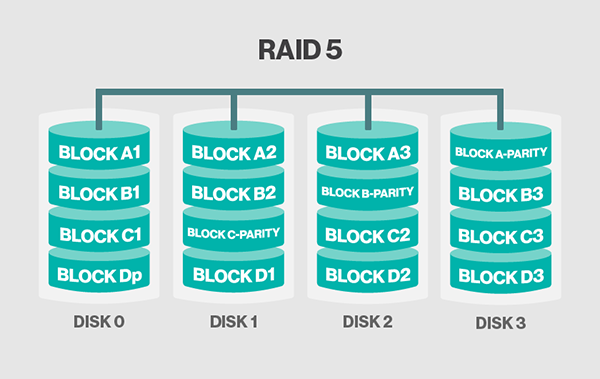
\includegraphics[scale=0.40]{img/raid55.png}\\
\caption{Sezionamento a livello di blocco con parit\`{a} distribuita\label{figura1.9} \cite{etichetta9}}
\end{figure}

\begin{figure}[htbp]
\item
\verb"RAID 6": livello simile a \verb"RAID 5", ma include un secondo schema di parit\`{a} distribuito attraverso le unit\`{a} nell'array. L'utilizzo di una parit\`{a} aggiuntiva consente all'array di continuare a funzionare anche se due dischi non funzionano contemporaneamente. Tuttavia, questa protezione supplementare \`{e} pi\`{u} costosa. Le matrici RAID \verb"6" hanno un costo superiore a gigabyte (GB) e spesso hanno prestazioni di scrittura pi\`{u} lente degli array \verb"RAID 5".\cite{etichetta9}\\

%http://www.webalice.it/climberjak/linux_informatica/gestione_dei_dischi_in_modo_ridondante.htm
\centering
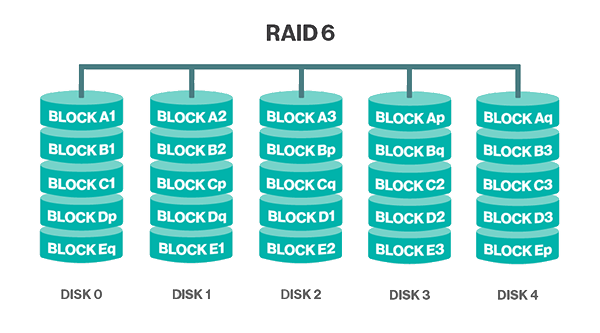
\includegraphics[scale=0.40]{img/raid66.png}\\
\caption{Sezionamento a livello di blocco con doppia parit\`{a} distribuita\label{figura1.10} \cite{etichetta9}}
\end{figure}
\end{itemize}


\paragraph{Livelli RAID Nidificati Annidati}

I livelli Annidati sono dei tipi di livelli pi\`{u} complessi ottenuti dalla combinazione di alcuni livelli RAID Standard. Esempi classici sono le configurazioni RAID \verb"0+1" o \verb"10".

%%%\textbf{spiegazione cinci -audio-}
%Nelle macchine non distribuite per garantire la ridondanza dei dati si scrive su piu dischi, sincrono (i dati vengono scritti simultaneamente) - come raid mirroring
%%%ci puo essere o un affarino (scheda) chiamato raid controller. Ha una memoria che puoi configurarlo.. puoi dirgli tra disco 1 e disco 2 imponi un raid 0. Quindi che succede? Da una macchina, cioe dal processore, tutte le volte che viene fatta una scrittura su disco, il raid controller la splitta e viene fatta in entrambi i dischi. quindi hai due dischi clonati (mirroring). Stessa cosa del REPLICA.

\item
\subsection{Codice di correzione errore (Erasure Coding)}
La codifica di cancellazione, noto come \emph{Erasure Coding} (EC) \`{e} un metodo di protezione dei dati, i quali vengono suddivisi in frammenti, estesi e codificati con pezzi di dati ridondanti e memorizzati su un insieme di posizioni o supporti di memorizzazione diversi.

L'obiettivo della codifica di cancellazione \`{e} quello di consentire di ricostruire i dati che vengono danneggiati utilizzando le informazioni sui dati memorizzati altrove nell'array. Lo svantaggio della codifica di cancellazione \`{e} che pu\`{o} essere pi\`{u} intenso della CPU e che pu\`{o} tradursi in una maggiore latenza.\cite{etichetta11}

La codifica di cancellazione \`{e} utile con la presenza di grandi quantit\`{a} di dati e tutte le applicazioni o sistemi che devono tollerare i guasti, come sistemi di array a dischi, griglie di dati, applicazioni di archiviazione distribuite. Un caso comune di utilizzo corrente per la codifica di cancellazione \`{e} in un sistema object-based cloud storage\cite{etichetta11}.

\subsubsection{Come funziona}
La codifica di cancellazione crea una funzione matematica per descrivere un insieme di numeri in modo che possano essere controllati per l'accuratezza e recuperati in caso di perdita. Questo \`{e} il concetto fondamentale dei metodi di codifica di cancellazione, implementati pi\`{u} frequentemente utilizzando i codici \textit{Reed-Solomon}\cite{etichetta11}. 

In termini matematici, la protezione offerta dalla codifica di cancellazione pu\`{o} essere rappresentata in forma semplice dalla seguente equazione:  
\begin{verbatim}
                       		n = k + m
\end{verbatim}
dove:
\begin{itemize}
\item 
la variabile \verb"k" \`{e} la quantit\`{a} originale di dati o simboli 
\item
la variabile \verb"m" indica i simboli aggiuntivi o ridondanti che vengono aggiunti per fornire protezione dai guasti
\item
la variabile \verb"n" \`{e} il numero totale di simboli creati dopo il processo di codifica di cancellazione\cite{etichetta11}
\item
la variabile \verb"r", chiamata velocit\`{a} di codice, \`{e} definita nel seguente modo: \\

						\verb"r = "\sqrt{\frac{k}{n}}
                       		
\end{itemize}

Ad esempio, in una configurazione \verb"10" di \verb"16", o EC \verb"10/16", sei simboli supplementari (\verb"m") saranno aggiunti ai \verb"10" simboli di base (\verb"k"). I \verb"16" frammenti di dati (\verb"n") saranno diffusi su \verb"16" unit\`{a}, nodi o posizioni geografiche. Il file originale potrebbe essere ricostruito da \verb"10" frammenti verificati.\cite{etichetta11}

I codici di cancellazione, noti anche come codici di correzione degli errori di avanzamento (FEC), sono stati sviluppati pi\`{u} di 50 anni fa. Da quel momento sono emersi diversi tipi. In uno dei tipi pi\`{u} comuni, \textit{Reed-Solomon}, i dati possono essere ricostruiti utilizzando qualsiasi combinazione di simboli \verb"k" o pezzi di dati, anche se i simboli \verb"m" sono persi o non sono disponibili. Ad esempio, in EC \verb"10/16", sei unit\`{a}, nodi o posizioni geografiche potrebbero essere persi o non disponibili e il file originale sar\`{a} ancora recuperabile.\cite{etichetta11}
 
\item
\section{Software utilizzato per gli esperimenti}
\item
\subsection{PosgreSQL}
PostgreSQL \`{e} un potente sistema \textit{Open Source} di database relazionale (DBMS, \textit{Database Management System}) cio\`{e} \`{e} un sistema software progettato per consentire la creazione e manipolazione efficiente di database, ovvero di collezioni di dati strutturati.\\ 
Ha pi\`{u} di \verb"15" anni di sviluppo attivo e un'architettura collaudata che ha guadagnato una notevole reputazione per l'affidabilit\`{a}, l'integrit\`{a} e la salvaguardia dei dati allocati e la correttezza di archiviazione.

PostgreSQL \`{e} un sistema di gestione dei database relazionale (\textit{Object-Relational}, acronimo ORDBMS) basato su POSTGRES, Versione 4.2, sviluppato presso l'Universit\`{a} della California presso il Dipartimento di Informatica di Berkeley.\cite{etichetta15}\\
Funziona su tutti i principali sistemi operativi, tra cui Linux, UNIX (AIX, BSD, HP-UX, SGI IRIX, Mac OS X, Solaris, Tru64), e Windows.\cite{etichetta15}\\

Supporta gran parte dello standard SQL e offre molte funzionalit\`{a} moderne:
\begin{itemize}
\item 
\textit{queries} complesse
\item
foreign keys
\item
triggers
\item
views aggiornabili
\item
integrit\`{a} transazionale
\item
controllo della concorrenza multiversione.
\end{itemize}

%Permette di aggiungere funzioni personalizzate sviluppate utilizzando diversi linguaggi di programmazione quali C/C++, Java, Perl, Python, Ruby, Tcl e Open Database Connectivity (ODBC).

Seguono le caratteristiche principali di PostgreSQL; le funzionalit\`{a} introdotte nella recente versione \verb"9.1" :
\begin{itemize}
\item 
elevata aderenza agli standard SQL;
\item 
architettura client-server con una gamma completa di driver e di client;
\item 
progettato in modo altamente concorrente, evitando che i processi in scrittura blocchino i processi in lettura;
\item 
altamente configurabile ed estendibile, consentendo svariati tipi di applicazioni;
\item 
elevate scalabilit\`{a} e prestazioni, unite a un ampio spettro di possibilit\`{a} per tarare la configurazione;
\item 
sofisticato ottimizzatore delle query, adeguato per la business intelligence;
\item 
supporto completo per Java, Python, Perl, PHP e molti altri linguaggi, sia per le procedure interne al server di database che per l'accesso da parte di client;
\item 
elevata affidabilit\`{a}, con una vasta serie di caratteristiche per durabilit\`{a} e alta disponibilit\`{a};
\item 
tipi di dati avanzati, come ad esempio GIS, full text search, e molti altri;
\item 
internazionalizzazione, codifiche multibyte e collation. \cite{etichetta12}
\end{itemize}\\

PostgreSQL \`{e} progettato per essere estensibile, poich\'{e} \`{e} possibile definire i propri tipi di dati, tipi di indici e lingue funzionali. Offre un ricco set di strumenti per gli sviluppatori in modo da gestire l'accesso simultaneo ai dati. Inoltre vi \`{e} la possibilit\`{a} di ottimizzarlo per soddisfare le proprie esigenze, tramite uno sviluppo di un plugin personalizzato.

Un database di classe enterprise, PostgreSQL vanta funzionalit\`{a} sofisticate come il controllo della concorrenza multiversione, il ripristino in tempo reale (\textit{point in time recovery}), \textit{tablespaces}, replica asincrona, transazioni nidificate (\textit{savepoints}), backup in linea/a caldo, un sofisticato query planner/optimizer, ed il \textit{write ahead logging} per una maggiore tolleranza ai guasti.\\
\`{E} estremamente scalabile sia nella quantit\`{a} pura di dati che pu\`{o} gestire sia nel numero di utenti concorrenti che pu\`{o} ospitare. Esistono sistemi Active PostgreSQL in	 ambienti di produzione che gestiscono oltre 4 terabyte di dati.\cite{etichetta15}

Alcuni limiti generali di PostgreSQL sono inclusi nei punti riportati di seguito:\\

\begin{tabular}{|l|l|r|}
%seconde parantesi 1cr se non vuoi linee e togli \hline
\hline
Dimensione massima del database & Illimitato\\
\hline
Dimensione massima Tabella & \verb"32 TB"\\
\hline
Dimensione massima Riga & \verb"1,6 TB"\\
\hline
Dimensione Massima campo & \verb"1 GB"\\
\hline
Numero Massimo Righe per tabella & Illimitato\\
\hline
Numero Massimo colonne per la tabella & \verb"250 - 1600"\\
%a seconda dei tipi di dati delle colonne\\
\hline
Numero Massimo indici per la tabella & Illimitato\cite{etichetta12}\\
\hline
\end{tabular}\\


MVCC (\textit{Multi-Version Concurrency Control}) \`{e} una tecnica avanzata per migliorare le prestazioni del database in un ambiente multiutente, mantenendo la coerenza dei dati. 
A differenza della maggior parte degli altri sistemi di database che utilizzano i \textit{locks} per il controllo della concorrenza, Postgres mantiene la coerenza dei dati utilizzando questo modello. Ci\`{o} significa che durante l'interrogazione di un database ogni transazione vede un'istantanea di dati (una versione del database), indipendentemente dallo stato corrente dei dati sottostanti. Questo protegge la transazione dalla visualizzazione di dati incoerenti che potrebbero essere causati da altri eventuali aggiornamenti simultanei delle transazioni sulle stesse righe di dati, fornendo l'isolamento della transazione per ciascuna sessione del database.

La differenza principale tra i modelli multiversione e di blocco \`{e} che nei blocchi MVCC acquisiti per la query (lettura) i dati non sono in conflitto con i blocchi acquisiti per la scrittura dei dati e quindi la lettura non blocca mai la scrittura e la scrittura non blocca mai la lettura.\cite{etichetta15}

\subsubsection{Caratteristiche PostgreSQL}
PostgreSQL ha il pieno supporto per le subquery (incluse sottotitoli nella clausola FROM), i livelli di isolamento delle transazioni di lettura e serializzabili. E mentre PostgreSQL ha un catalogo di sistema completamente relazionale che supporta pi\`{u} schemi per database, il suo catalogo \`{e} accessibile anche attraverso lo schema di informazioni definito nello standard SQL.

Le funzionalit\`{a} di integrit\`{a} dei dati includono le chiavi primarie (combinate), le chiavi estranee con aggiornamenti e cancellazioni a cascata, i controlli dei vincoli, i vincoli unici e non i vincoli nullo.

Ha anche una serie di estensioni e funzionalit\`{a} avanzate. PostgreSQL supporta indici composti, unici, parziali e funzionali che possono utilizzare qualsiasi metodo di archiviazione B-tree, R-tree, hash o GiST.

Altre funzionalit\`{a} avanzate includono l'ereditariet\`{a} delle tabelle, i sistemi di regole e gli eventi del database. L'ereditarietà di tabella mette un orientamento orientato all'oggetto sulla creazione della tabella, consentendo ai progettisti di database di derivare nuove tabelle da altre tabelle, trattandole come classi di base. Ancora meglio, PostgreSQL supporta sia l'ereditarietà singola che quella multipla in questo modo.

Il sistema di regole, chiamato anche il sistema di riscrittura delle query, consente al progettista del database di creare regole che identificano operazioni specifiche per una determinata tabella o vista e le trasformano dinamicamente in operazioni alternative quando vengono elaborate.

Il sistema eventi \`{e} un sistema di comunicazione interprocesso in cui i messaggi e gli eventi possono essere trasmessi tra i client utilizzando i comandi \verb"LISTEN" e \verb"NOTIFY", consentendo sia la semplice comunicazione peer to peer sia un coordinamento avanzato sugli eventi del database. Poich\'{e} le notifiche possono essere rilasciate da trigger e stored procedure, i client PostgreSQL possono monitorare eventi di database come gli aggiornamenti, gli \verb"insert" o le eliminazioni di tabella quando vengono eseguiti.\cite{etichetta15}

\subsubsection{Elevata personalizzazione}
PostgreSQL esegue procedure memorizzate in pi\`{u} di una dozzina di linguaggi di programmazione, tra cui Java, Perl, Python, Ruby, Tcl, C / C ++ e il proprio PL / pgSQL, simile a PL / SQL di Oracle. I trigger e le stored procedure possono essere scritti in C e caricati nel database come libreria, permettendo una grande flessibilit\`{a} nell'estensione delle sue funzionalit\`{a}. Allo stesso modo, PostgreSQL include un \textit{framework} che consente agli sviluppatori di definire e creare i propri tipi di dati personalizzati insieme a funzioni di supporto e operatori che definiscono il loro comportamento.

Il codice sorgente di PostgreSQL \`{e} disponibile sotto una licenza libera open source: la licenza PostgreSQL. Questa licenza d\`{a} la libert\`{a} di utilizzare, modificare e distribuire PostgreSQL in qualsiasi forma, sorgente aperta o chiusa.\cite{etichetta15}

%Ci sono molti approcci disponibili per scalare PostgreSQL oltre l'esecuzione su un singolo server. Una descrizione della terminologia e delle tecnologie di base coinvolte è quella di Alta disponibilità e bilanciamento del carico. C'è una presentazione che copre alcune di queste soluzioni.
Non esiste un unico formato per tutti i software di replica. \`{E} necessario capire le proprie esigenze e come si adattino diversi approcci. Ad esempio, ecco due estremi nello spazio del problema di replica:
Hai alcuni server collegati a una rete locale che vuoi mantenere sempre la corrente per scopi di failover e di bilanciamento del carico. Qui si considererebbero soluzioni sincrone, desiderose e quindi prive di conflitti.
I tuoi utenti prendono una copia locale del database con loro sui computer portatili quando lasciano l'ufficio, apportano modifiche mentre sono lontani e hanno bisogno di unire quelli con il database principale quando tornano. Qui si desidera un approccio asincrono e pigro di replica e sarà costretto a considerare come gestire i conflitti nei casi in cui lo stesso record sia stato modificato sia sul server master che su una copia locale.
Questi sono problemi di replica del database, ma il modo migliore per risolverli è molto diverso. E come si può vedere da questi esempi, la replica ha molte terminologie specifiche che dovrai capire per capire quale classe di soluzione ha senso per i tuoi requisiti. Una grande fonte per questo sfondo è nelle Termini e definizioni di Postgres-R per la replica del database. L'argomento principale teorico che non menziona è come risolvere la risoluzione dei conflitti nei casi di pigri repliche come la situazione del computer portatile, che riguarda il voto e simili schemi.

Hot Standby / Streaming Replication è disponibile a partire da PostgreSQL 9.0 e fornisce una replica binaria asincrona a uno o più standby. Gli standby possono anche diventare standbys caldi, che possono essere richiesti come database di sola lettura. Questo è il tipo di replica più veloce disponibile in quanto i dati WAL vengono inviati immediatamente piuttosto che aspettare che un intero segmento venga prodotto e spedito.
Warm Standby / Log Spedizione è una soluzione HA che replica un cluster di database ad un archivio o un caldo (può essere portato in fretta, ma non disponibile per la query) server standby. Il sovraccarico è molto basso e è facile da installare. Questa è una soluzione semplice e appropriata se tutto ciò che ti interessa è un backup continuo e brevi tempi di failover.
L'estrazione Logical Changeset di PostgreSQL 9.4 forma il fondamento della funzionalità di replica di reazione bidirezionale e Log Log Logging Streaming che viene aggiunto a PostgreSQL.
Storicamente, il team di base di PostgreSQL ha considerato la tecnologia di replica e clustering al di fuori dell'ambito del focus del progetto principale, ma questo è cambiato nel 2008, vedere l'istruzione del Team Core. La replica è ora un focus significativo dello sviluppo continuativo

\textbf{(spiegazione cinci -audio-)}
%Uno dei punti di forza che ha reso famoso e versatile Posgres è che è un (Database Management System è un sistema software progettato per consentire la creazione e manipolazione efficiente di database (ovvero di collezioni di dati strutturati) ) (scritto in C). Ha dei rametti dove te riesci ad agganciarci dei software fatti ad OC. te ti agganci a un sistema di segnalistica interna e lui quindi tramite messaggi di scambio interno ti permette di lavorare (ti dice "ho fatto l'inserimento di questa tabella(INSERT), ti scatta il segnale, e te riesci a intercettare e quindi fare delle operazioni)

%Pg Logical è un estensione di Posgres. Lui capisce quando fa inserimenti e riesce a duplicare soltando parti di database. Mentre replica di posgres per adesso ti replicherebbe tutto il DB. Invece noi si fa con solo tabelle (R) o quanti record di tabelle (per id maggiori di x) adirittura si vogliono replicare o colonne di tabelle \\

La replica delle modifiche dello schema \`{e} un problema frequentemente discusso e solo pochi sistemi di database forniscono le estensioni necessarie per implementarlo. PostgreSQL non fornisce la possibilit\`{a} di definire i trigger richiamati sulle modifiche dello schema, quindi un modo trasparente per replicare le modifiche dello schema non \`{e} possibile senza un sostanziale lavoro nel sistema centrale di PostgreSQL.
Invece tendono ad essere gruppi di istruzioni DDL e DML che modificano pi\`{u} oggetti di database e fanno manipolazioni di dati di massa come l'aggiornamento di una nuova colonna al suo valore iniziale.
Il sistema di replica Pglogical avr\`{a} un meccanismo per eseguire script SQL in modo controllato come parte del processo di replica.

\item
\subsubsection{Write-Ahead Loggin (WAL)}
\textit{Write-Ahead Logging} (WAL) \`{e} un metodo standard per garantire l'integrit\`{a} dei dati. Il concetto centrale di WAL \`{e} che le modifiche ai file di dati (dove risiedono tabelle e indici) devono essere scritte solo dopo che tali modifiche sono state registrate, ovvero dopo che i record di registro che descrivono le modifiche sono stati scaricati nella memoria permanente. Se viene seguita questa procedura, non abbiamo bisogno di svuotare le pagine di dati sul disco su ogni \textit{commit} di transazione, perch\'{e} sappiamo che in caso di crash saremo in grado di recuperare il database usando il log: eventuali modifiche che non sono state applicate alle pagine di dati possono essere rifatte dai record del registro. Questo \`{e} il recupero \textit{roll-forward}, noto anche come REDO.\\

Poich\'{e} WAL ripristina il contenuto del file di database dopo un arresto anomalo, i \textit{filesystem} registrati non sono necessari per l'archiviazione affidabile dei file di dati o dei file WAL. \\
%In effetti, l'overhead del journaling può ridurre le prestazioni, specialmente se l'inserimento nel journal fa sì che i dati del file system vengano scaricati su disco. Fortunatamente, lo svuotamento dei dati durante l'inserimento nel journal può spesso essere disabilitato con un'opzione di montaggio del file system, ad es. data = writeback su un file system Linux ext3. I file system journalizzati migliorano la velocità di avvio dopo un arresto anomalo.
L'utilizzo di WAL determina un numero notevolmente ridotto di scritture su disco, poich\'{e} \`{e} necessario scaricare il file di registro sul disco per garantire che una transazione venga eseguita, piuttosto che ogni file di dati modificato dalla transazione. \\
Il file di registro viene scritto in modo sequenziale e pertanto il costo della sincronizzazione del log \`{e} molto inferiore al costo dello svuotamento delle pagine di dati. Ci\`{o} \`{e} particolarmente vero per i server che gestiscono molte piccole transazioni toccando diverse parti dell'archivio dati. Inoltre, quando il server sta elaborando molte piccole transazioni simultanee, un \verb"fsync" del file di log pu\`{o} essere sufficiente per il \textit{commit} di molte transazioni.\cite{etichetta15}

Archiviando i dati WAL possiamo supportare il ripristino in qualsiasi istante dei dati WAL disponibili: installiamo semplicemente un backup fisico preliminare del database e riproduciamo il registro WAL fino al momento desiderato. Inoltre, il backup fisico non deve essere un'istantanea istantanea dello stato del database: se viene eseguito per un certo periodo di tempo, la riproduzione del log WAL per quel periodo risolver\`{a} eventuali incoerenze interne.\textbf{vedere se metterlo}

\item 
\subsubsection{File di configurazione di PostgreSQL}
Segue parte del file di configurazione di PostgreSQL chiamato \verb"postgresql.conf" ottenuta dall'ultima versione \verb"10.0", ponendo attenzione ai parametri dei lanci di configurazione:
\\ 

\vspace{-0.5cm}
\begin{verbatim}
 
# -----------------------------
# PostgreSQL configuration file
# -----------------------------
#
# This file consists of lines of the form:
#
#   name = value
#
# (The "=" is optional.)  Whitespace may be used.  Comments are introduced with
# "#" anywhere on a line.  The complete list of parameter names and allowed
# values can be found in the PostgreSQL documentation.
#
# The commented-out settings shown in this file represent the default values.
# Re-commenting a setting is NOT sufficient to revert it to the default value;
# you need to reload the server.
#
# This file is read on server startup and when the server receives a SIGHUP
# signal.  If you edit the file on a running system, you have to SIGHUP the
# server for the changes to take effect, run "pg_ctl reload", or execute
# "SELECT pg_reload_conf()".  Some parameters, which are marked below,
# require a server shutdown and restart to take effect.
#
# Any parameter can also be given as a command-line option to the server, e.g.,
# "postgres -c log_connections=on".  Some parameters can be changed at run time
# with the "SET" SQL command.
#
# Memory units:  kB = kilobytes        Time units:  ms  = milliseconds
#                MB = megabytes                     s   = seconds
#                GB = gigabytes                     min = minutes
#                TB = terabytes                     h   = hours
#                                                   d   = days


#------------------------------------------------------------------------------
# FILE LOCATIONS
#------------------------------------------------------------------------------

# The default values of these variables are driven from the -D command-line
# option or PGDATA environment variable, represented here as ConfigDir.

#data_directory = 'ConfigDir'		# use data in another directory
					# (change requires restart)
#hba_file = 'ConfigDir/pg_hba.conf'	# host-based authentication file
					# (change requires restart)
#ident_file = 'ConfigDir/pg_ident.conf'	# ident configuration file
					# (change requires restart)

# If external_pid_file is not explicitly set, no extra PID file is written.
#external_pid_file = ''			# write an extra PID file
					# (change requires restart)


#------------------------------------------------------------------------------
# CONNECTIONS AND AUTHENTICATION
#------------------------------------------------------------------------------

# - Connection Settings -

listen_addresses = '*'			# what IP address(es) to listen on;
					# comma-separated list of addresses;
					# defaults to 'localhost'; use '*' for all
					# (change requires restart)
port = 5432				# (change requires restart)
max_connections = 100			# (change requires restart)
#superuser_reserved_connections = 3	# (change requires restart)
#unix_socket_directories = '/tmp'	# comma-separated list of directories
					# (change requires restart)
#unix_socket_group = ''			# (change requires restart)
#unix_socket_permissions = 0777		# begin with 0 to use octal notation
					# (change requires restart)
#bonjour = off				# advertise server via Bonjour
					# (change requires restart)
#bonjour_name = ''			# defaults to the computer name
					# (change requires restart)

# - Security and Authentication -

#authentication_timeout = 1min		# 1s-600s
#ssl = off
#ssl_ciphers = 'HIGH:MEDIUM:+3DES:!aNULL' # allowed SSL ciphers
#ssl_prefer_server_ciphers = on
#ssl_ecdh_curve = 'prime256v1'
#ssl_dh_params_file = ''
#ssl_cert_file = 'server.crt'
#ssl_key_file = 'server.key'
#ssl_ca_file = ''
#ssl_crl_file = ''
#password_encryption = md5		# md5 or scram-sha-256
#db_user_namespace = off
#row_security = on

# GSSAPI using Kerberos
#krb_server_keyfile = ''
#krb_caseins_users = off

# - TCP Keepalives -
# see "man 7 tcp" for details

#tcp_keepalives_idle = 0		# TCP_KEEPIDLE, in seconds;
					# 0 selects the system default
#tcp_keepalives_interval = 0		# TCP_KEEPINTVL, in seconds;
					# 0 selects the system default
#tcp_keepalives_count = 0		# TCP_KEEPCNT;
					# 0 selects the system default


#------------------------------------------------------------------------------
# RESOURCE USAGE (except WAL)
#------------------------------------------------------------------------------

# - Memory -

shared_buffers = 256MB			# min 128kB
					# (change requires restart)
#huge_pages = try			# on, off, or try
					# (change requires restart)
#temp_buffers = 8MB			# min 800kB
max_prepared_transactions = 100		# zero disables the feature
					# (change requires restart)
# Caution: it is not advisable to set max_prepared_transactions nonzero unless
# you actively intend to use prepared transactions.
#work_mem = 32MB				# min 64kB
#maintenance_work_mem = 128MB		# min 1MB
#replacement_sort_tuples = 150000	# limits use of replacement selection sort
#autovacuum_work_mem = -1		# min 1MB, or -1 to use maintenance_work_mem
#max_stack_depth = 2MB			# min 100kB
dynamic_shared_memory_type = posix	# the default is the first option
					# supported by the operating system:
					#   posix
					#   sysv
					#   windows
					#   mmap
					# use none to disable dynamic shared memory
					# (change requires restart)

# - Disk -

#temp_file_limit = -1			# limits per-process temp file space
					# in kB, or -1 for no limit

# - Kernel Resource Usage -

#max_files_per_process = 1000		# min 25
					# (change requires restart)
shared_preload_libraries = 'pglogical'		# (change requires restart)

# - Cost-Based Vacuum Delay -

#vacuum_cost_delay = 0			# 0-100 milliseconds
#vacuum_cost_page_hit = 1		# 0-10000 credits
#vacuum_cost_page_miss = 10		# 0-10000 credits
#vacuum_cost_page_dirty = 20		# 0-10000 credits
#vacuum_cost_limit = 200		# 1-10000 credits

# - Background Writer -

#bgwriter_delay = 200ms			# 10-10000ms between rounds
#bgwriter_lru_maxpages = 100		# 0-1000 max buffers written/round
#bgwriter_lru_multiplier = 2.0		# 0-10.0 multiplier on buffers scanned/round
#bgwriter_flush_after = 512kB		# measured in pages, 0 disables

# - Asynchronous Behavior -

#effective_io_concurrency = 1		# 1-1000; 0 disables prefetching
max_worker_processes = 64		# (change requires restart)
#max_parallel_workers_per_gather = 2	# taken from max_parallel_workers
#max_parallel_workers = 8		# maximum number of max_worker_processes that
					# can be used in parallel queries
#old_snapshot_threshold = -1		# 1min-60d; -1 disables; 0 is immediate
					# (change requires restart)
#backend_flush_after = 0		# measured in pages, 0 disables


#------------------------------------------------------------------------------
# WRITE AHEAD LOG
#------------------------------------------------------------------------------

# - Settings -

wal_level = logical			# minimal, archive, hot_standby, or logical
					# (change requires restart)
#fsync = on				# turns forced synchronization on or off
synchronous_commit = off		# synchronization level;
														# off, local, remote_write, or on
#wal_sync_method = fsync		# the default is the first option
					# supported by the operating system:
					#   open_datasync
					#   fdatasync (default on Linux)
					#   fsync
					#   fsync_writethrough
					#   open_sync
#full_page_writes = on			# recover from partial page writes
#wal_compression = off			# enable compression of full-page writes
#wal_log_hints = off			# also do full page writes of non-critical updates
					# (change requires restart)
#wal_buffers = -1			# min 32kB, -1 sets based on shared_buffers
					# (change requires restart)
#wal_writer_delay = 200ms		# 1-10000 milliseconds
#wal_writer_flush_after = 1MB		# measured in pages, 0 disables

#commit_delay = 0			# range 0-100000, in microseconds
#commit_siblings = 5			# range 1-1000

# - Checkpoints -

#checkpoint_timeout = 5min		# range 30s-1d
#max_wal_size = 1GB
#min_wal_size = 80MB
#checkpoint_completion_target = 0.5	# checkpoint target duration, 0.0 - 1.0
#checkpoint_flush_after = 256kB		# measured in pages, 0 disables
#checkpoint_warning = 30s		# 0 disables

# - Archiving -

#archive_mode = off		# enables archiving; off, on, or always
				# (change requires restart)
#archive_command = ''		# command to use to archive a logfile segment
				# placeholders: %p = path of file to archive
				#               %f = file name only
				# e.g. 'test ! -f /mnt/server/archivedir/%f && cp %p /mnt/server/archivedir/%f'
#archive_timeout = 0		# force a logfile segment switch after this
				# number of seconds; 0 disables


#------------------------------------------------------------------------------
# REPLICATION
#------------------------------------------------------------------------------

# - Sending Server(s) -

# Set these on the master and on any standby that will send replication data.

max_wal_senders = 64		# max number of walsender processes
				# (change requires restart)
#wal_keep_segments = 0		# in logfile segments, 16MB each; 0 disables
#wal_sender_timeout = 60s	# in milliseconds; 0 disables

max_replication_slots = 64	# max number of replication slots
				# (change requires restart)
track_commit_timestamp = on	# collect timestamp of transaction commit
				# (change requires restart)

# - Master Server -

# These settings are ignored on a standby server.

synchronous_standby_names = '1 (r1, r2, r3, r4)'
				# standby servers that provide sync rep
				# method to choose sync standbys, number of sync standbys,
				# and comma-separated list of application_name
				# from standby(s); '*' = all
#vacuum_defer_cleanup_age = 0	# number of xacts by which cleanup is delayed

# - Standby Servers -

# These settings are ignored on a master server.

#hot_standby = on			# "off" disallows queries during recovery
					# (change requires restart)
#max_standby_archive_delay = 30s	# max delay before canceling queries
					# when reading WAL from archive;
					# -1 allows indefinite delay
#max_standby_streaming_delay = 30s	# max delay before canceling queries
					# when reading streaming WAL;
					# -1 allows indefinite delay
#wal_receiver_status_interval = 10s	# send replies at least this often
					# 0 disables
#hot_standby_feedback = off		# send info from standby to prevent
					# query conflicts
#wal_receiver_timeout = 60s		# time that receiver waits for
					# communication from master
					# in milliseconds; 0 disables
#wal_retrieve_retry_interval = 5s	# time to wait before retrying to
					# retrieve WAL after a failed attempt

# - Subscribers -

# These settings are ignored on a publisher.

max_logical_replication_workers =  16 #4	# taken from max_worker_processes
					# (change requires restart)
#max_sync_workers_per_subscription = 2	# taken from max_logical_replication_workers


#------------------------------------------------------------------------------
# QUERY TUNING
#------------------------------------------------------------------------------

# - Planner Method Configuration -

#enable_bitmapscan = on
#enable_hashagg = on
#enable_hashjoin = on
#enable_indexscan = on
#enable_indexonlyscan = on
#enable_material = on
#enable_mergejoin = on
#enable_nestloop = on
#enable_seqscan = on
#enable_sort = on
#enable_tidscan = on

# - Planner Cost Constants -

#seq_page_cost = 1.0			# measured on an arbitrary scale
#random_page_cost = 4.0			# same scale as above
#cpu_tuple_cost = 0.01			# same scale as above
#cpu_index_tuple_cost = 0.005		# same scale as above
#cpu_operator_cost = 0.0025		# same scale as above
#parallel_tuple_cost = 0.1		# same scale as above
#parallel_setup_cost = 1000.0	# same scale as above
#min_parallel_table_scan_size = 8MB
#min_parallel_index_scan_size = 512kB
#effective_cache_size = 4GB

# - Genetic Query Optimizer -

#geqo = on
#geqo_threshold = 12
#geqo_effort = 5			# range 1-10
#geqo_pool_size = 0			# selects default based on effort
#geqo_generations = 0			# selects default based on effort
#geqo_selection_bias = 2.0		# range 1.5-2.0
#geqo_seed = 0.0			# range 0.0-1.0

# - Other Planner Options -

#default_statistics_target = 100	# range 1-10000
#constraint_exclusion = partition	# on, off, or partition
#cursor_tuple_fraction = 0.1		# range 0.0-1.0
#from_collapse_limit = 8
#join_collapse_limit = 8		# 1 disables collapsing of explicit
					# JOIN clauses
#force_parallel_mode = off


#------------------------------------------------------------------------------
# ERROR REPORTING AND LOGGING
#------------------------------------------------------------------------------

# - Where to Log -

#log_destination = 'stderr'		# Valid values are combinations of
					# stderr, csvlog, syslog, and eventlog,
					# depending on platform.  csvlog
					# requires logging_collector to be on.

# This is used when logging to stderr:
#logging_collector = off		# Enable capturing of stderr and csvlog
					# into log files. Required to be on for
					# csvlogs.
					# (change requires restart)

# These are only used if logging_collector is on:
#log_directory = 'log'			# directory where log files are written,
					# can be absolute or relative to PGDATA
#log_filename = 'postgresql-%Y-%m-%d_%H%M%S.log'	# log file name pattern,
					# can include strftime() escapes
#log_file_mode = 0600			# creation mode for log files,
					# begin with 0 to use octal notation
#log_truncate_on_rotation = off		# If on, an existing log file with the
					# same name as the new log file will be
					# truncated rather than appended to.
					# But such truncation only occurs on
					# time-driven rotation, not on restarts
					# or size-driven rotation.  Default is
					# off, meaning append to existing files
					# in all cases.
#log_rotation_age = 1d			# Automatic rotation of logfiles will
					# happen after that time.  0 disables.
#log_rotation_size = 10MB		# Automatic rotation of logfiles will
					# happen after that much log output.
					# 0 disables.

# These are relevant when logging to syslog:
#syslog_facility = 'LOCAL0'
#syslog_ident = 'postgres'
#syslog_sequence_numbers = on
#syslog_split_messages = on

# This is only relevant when logging to eventlog (win32):
# (change requires restart)
#event_source = 'PostgreSQL'

# - When to Log -

#client_min_messages = notice		# values in order of decreasing detail:
					#   debug5
					#   debug4
					#   debug3
					#   debug2
					#   debug1
					#   log
					#   notice
					#   warning
					#   error

#log_min_messages = warning		# values in order of decreasing detail:
					#   debug5
					#   debug4
					#   debug3
					#   debug2
					#   debug1
					#   info
					#   notice
					#   warning
					#   error
					#   log
					#   fatal
					#   panic

#log_min_error_statement = error	# values in order of decreasing detail:
					#   debug5
					#   debug4
					#   debug3
					#   debug2
					#   debug1
					#   info
					#   notice
					#   warning
					#   error
					#   log
					#   fatal
					#   panic (effectively off)

#log_min_duration_statement = -1	# -1 is disabled, 0 logs all statements
					# and their durations, > 0 logs only
					# statements running at least this number
					# of milliseconds


# - What to Log -

#debug_print_parse = off
#debug_print_rewritten = off
#debug_print_plan = off
#debug_pretty_print = on
#log_checkpoints = off
#log_connections = off
#log_disconnections = off
#log_duration = off
#log_error_verbosity = default		# terse, default, or verbose messages
#log_hostname = off
#log_line_prefix = '%m [%p] '		# special values:
					#   %a = application name
					#   %u = user name
					#   %d = database name
					#   %r = remote host and port
					#   %h = remote host
					#   %p = process ID
					#   %t = timestamp without milliseconds
					#   %m = timestamp with milliseconds
					#   %n = timestamp with milliseconds (as a Unix epoch)
					#   %i = command tag
					#   %e = SQL state
					#   %c = session ID
					#   %l = session line number
					#   %s = session start timestamp
					#   %v = virtual transaction ID
					#   %x = transaction ID (0 if none)
					#   %q = stop here in non-session
					#        processes
					#   %% = '%'
					# e.g. '<%u%%%d> '
#log_lock_waits = off			# log lock waits >= deadlock_timeout
#log_statement = 'none'			# none, ddl, mod, all
#log_replication_commands = off
#log_temp_files = -1			# log temporary files equal or larger
					# than the specified size in kilobytes;
					# -1 disables, 0 logs all temp files
log_timezone = 'UTC'


# - Process Title -

#cluster_name = ''			# added to process titles if nonempty
					# (change requires restart)
#update_process_title = on


#------------------------------------------------------------------------------
# RUNTIME STATISTICS
#------------------------------------------------------------------------------

# - Query/Index Statistics Collector -

#track_activities = on
#track_counts = on
#track_io_timing = off
#track_functions = none			# none, pl, all
#track_activity_query_size = 1024	# (change requires restart)
#update_process_title = on
#stats_temp_directory = 'pg_stat_tmp'


# - Statistics Monitoring -

#log_parser_stats = off
#log_planner_stats = off
#log_executor_stats = off
#log_statement_stats = off


#------------------------------------------------------------------------------
# AUTOVACUUM PARAMETERS
#------------------------------------------------------------------------------

#autovacuum = on			# Enable autovacuum subprocess?  'on'
					# requires track_counts to also be on.
#log_autovacuum_min_duration = -1	# -1 disables, 0 logs all actions and
					# their durations, > 0 logs only
					# actions running at least this number
					# of milliseconds.
#autovacuum_max_workers = 3		# max number of autovacuum subprocesses
					# (change requires restart)
#autovacuum_naptime = 1min		# time between autovacuum runs

# - Statement Behavior -

#search_path = '"$user", public'	# schema names
#default_tablespace = ''		# a tablespace name, '' uses the default
#temp_tablespaces = ''			# a list of tablespace names, '' uses
					# only default tablespace
#check_function_bodies = on
#default_transaction_isolation = 'read committed'
#default_transaction_read_only = off
#default_transaction_deferrable = off
#session_replication_role = 'origin'
#statement_timeout = 0			# in milliseconds, 0 is disabled
#lock_timeout = 0			# in milliseconds, 0 is disabled
#idle_in_transaction_session_timeout = 0	# in milliseconds, 0 is disabled
#vacuum_freeze_min_age = 50000000
#vacuum_freeze_table_age = 150000000
#vacuum_multixact_freeze_min_age = 5000000
#vacuum_multixact_freeze_table_age = 150000000
#bytea_output = 'hex'			# hex, escape
#xmlbinary = 'base64'
#xmloption = 'content'
#gin_fuzzy_search_limit = 0
#gin_pending_list_limit = 4MB

# - Locale and Formatting -

datestyle = 'iso, mdy'
#intervalstyle = 'postgres'
timezone = 'UTC'
#timezone_abbreviations = 'Default'     # Select the set of available time zone
					# abbreviations.  Currently, there are
					#   Default
					#   Australia (historical usage)
					#   India
					# You can create your own file in
					# share/timezonesets/.
#extra_float_digits = 0			# min -15, max 3
#client_encoding = sql_ascii		# actually, defaults to database
					# encoding

# These settings are initialized by initdb, but they can be changed.
lc_messages = 'C'			# locale for system error message
					# strings
lc_monetary = 'C'			# locale for monetary formatting
lc_numeric = 'C'			# locale for number formatting
lc_time = 'C'				# locale for time formatting

# default configuration for text search
default_text_search_config = 'pg_catalog.english'

# - Other Defaults -

#dynamic_library_path = '/cyone1/postgres10/usr/lib/postgresql/'
#local_preload_libraries = ''
#session_preload_libraries = ''


#------------------------------------------------------------------------------
# LOCK MANAGEMENT
#------------------------------------------------------------------------------

#deadlock_timeout = 1s
#max_locks_per_transaction = 64		# min 10
					# (change requires restart)
#max_pred_locks_per_transaction = 64	# min 10
					# (change requires restart)
#max_pred_locks_per_relation = -2	# negative values mean
					# (max_pred_locks_per_transaction
					#  / -max_pred_locks_per_relation) - 1
#max_pred_locks_per_page = 2            # min 0


#------------------------------------------------------------------------------
# VERSION/PLATFORM COMPATIBILITY
#------------------------------------------------------------------------------

# - Previous PostgreSQL Versions -

#array_nulls = on
#backslash_quote = safe_encoding	# on, off, or safe_encoding
#default_with_oids = off
#escape_string_warning = on
#lo_compat_privileges = off
#operator_precedence_warning = off
#quote_all_identifiers = off
#sql_inheritance = on
#standard_conforming_strings = on
#synchronize_seqscans = on

# - Other Platforms and Clients -

#transform_null_equals = off


#------------------------------------------------------------------------------
# ERROR HANDLING
#------------------------------------------------------------------------------

#exit_on_error = off			# terminate session on any error?
#restart_after_crash = on		# reinitialize after backend crash?


#------------------------------------------------------------------------------
# CONFIG FILE INCLUDES
#------------------------------------------------------------------------------

# These options allow settings to be loaded from files other than the
# default postgresql.conf.

#include_dir = 'conf.d'			# include files ending in '.conf' from
					# directory 'conf.d'
#include_if_exists = 'exists.conf'	# include file only if it exists
#include = 'special.conf'		# include file


#------------------------------------------------------------------------------
# CUSTOMIZED OPTIONS
#------------------------------------------------------------------------------

# Add settings for extensions here



pglogical.conflict_resolution = 'last_update_wins'
\end{verbatim}
 \vspace{-0.3cm}
 
\item
\subsection{Pglogical}
Pglogical \`{e} un sistema logico di replica implementato come estensione di PostgreSQL. Completamente integrato, non richiede alcun triggers o programmi esterni. Questa alternativa alla replica fisica \`{e} un metodo altamente efficiente per replicare i dati utilizzando un modello di \textit{publish/subscribe} per la replica selettiva.\cite{etichetta3}
%Metodo di replicazione : Master-Slave

\subsubsection{Vantaggi}
I vantaggi offerti da Pglogical sono i seguenti:
\begin{itemize}
\item
Replica sincrona
\item
Replica ritardata
\item
Risoluzione dei conflitti configurabili
\item
Capacit\`{a} di convertire lo standby fisico in una replica logica
\item
Pu\`{o} pubblicare i dati da PostgreSQL a un abbonato Postgres-XL
\item
Le sequenze possono essere replicate
\item
Nessun trigger significa ridurre il carico di scrittura sul Provider
\item
Nessuna re-esecuzione di SQL significa overhead e latenza ridotti per il Sottoscrittore
\item
Il sottoscrittore non \`{e} in ripristino di riposo caldo, in modo da poter utilizzare tavoli temp, non sbloccati o normali
\item
Non \`{e} necessario annullare le query per consentire alla replica di continuare la riproduzione
\item
Il sottoscrittore (\textit{subscriber}) pu\`{o} avere diversi utenti e protezione, indici diversi, impostazioni di parametri diversi
\item
Replica solo un database o un sottoinsieme di tabelle, noto come set di replica (\textit{Replication Sets})
\item
Replicare in versioni o architetture di PostgreSQL, consentendo aggiornamenti a bassa o zero-downtime
\item
Pi\`{u} server a monte in un singolo subscriber per l'accumulo di cambiamenti.\cite{etichetta3}
\end{itemize}

\subsubsection{Casi di uso}
I diagrammi che seguono descrivono i gestori di database delle funzioni che sono in grado di eseguire con pglogical:

\begin{figure}[htbp]
\centering
Migrare e aggiornare PostgreSQL con tempi di inattivit\`{a} quasi a zero
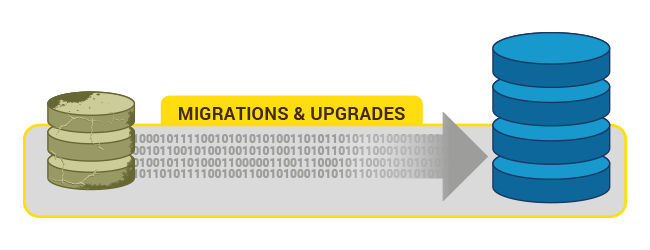
\includegraphics[scale=0.70]{img/pglogical_1.png}\\

\caption{Migrazione e aggiornamenti PostgreSQL \label{figura1} \cite{etichetta3}}

Accumulare le modifiche provenienti da server di database scartati in un data warehouse
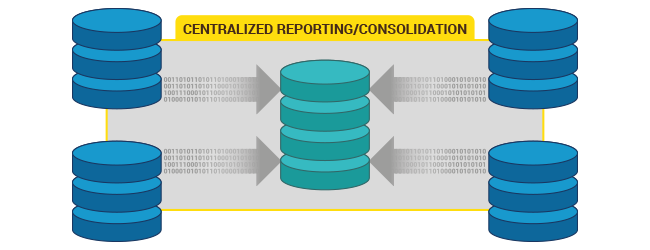
\includegraphics[scale=0.70]{img/pglogical_2.png}\\

\caption{Aggregazione \label{figura2} \cite{etichetta3}}
\end{figure}

\begin{figure}[htbp]
\centering
Copiare tutti o una selezione di tabelle di database ad altri nodi di un cluster
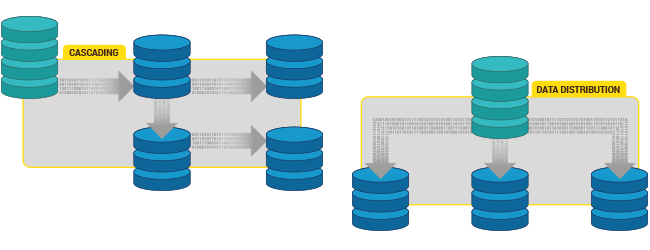
\includegraphics[scale=0.70]{img/pglogical_3.png}\\

\caption{A cascata e distribuzione dati \label{figura3} \cite{etichetta3}}
Le modifiche del database in tempo reale ad altri sistemi
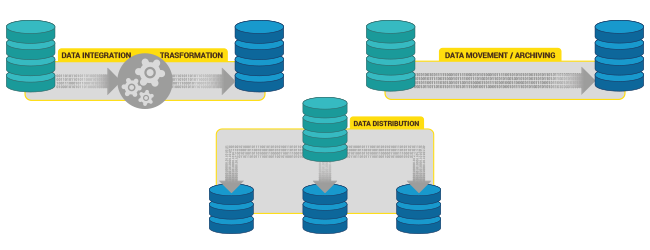
\includegraphics[scale=0.70]{img/pglogical_4.png}\\

\caption{A cascata e distribuzione dati \label{figura4} \cite{etichetta3}}
\end{figure}

\subsubsection{Come funziona pglogical?}
Pglogical utilizza le funzioni di Decodifica Logica aggiunte da 2ndQuadrant (e disponibili da PostgreSQL 9.4). Pglogical funziona ancora pi\`{u} veloce con PostgreSQL 9.5 e successive, con bassi overhead su entrambi i provider e abbonati.

Pglogical si basa molto sulle caratteristiche introdotte nell'ambito dello sviluppo BDR, tra cui:

\begin{itemize}
\item
Decodifica logica
\item
\item
Slot di replica
\item
Lavoratori di sfondo statico
\item
Origini di replica
\item
Impegnano timestamp
\item
Messaggi WAL logici.\cite{etichetta3}
\end{itemize}

\subsubsection{Replica pglogical Bi-Directional Replication (BDR)?}
No. pglogical non fornisce funzionalità complete di replica multi-master e un supporto di modifica dello schema coerente, come fa la BDR. Pglogical incorpora le funzionalità di BDR e le lezioni apprese da BDR per produrre una soluzione più semplice e più semplice da utilizzare per la replica unidirezionale, utilizzabile da più persone per una vasta gamma di casi di utilizzo. BDR è stato progettato innanzitutto per il multi-master della rete a n-way, e questo è stato difficile adattarsi bene alla replica mono-master a senso unico.

Lo sviluppo di BDR continuerà per quelli che richiedono piena capacità multi-master, riutilizzando gran parte del codice da pglogical.\cite{etichetta3}


\texttt{DA METTERE? DIFFERENZA TRA PG LOGICAL E BDR}
Replica pglogical Bi-Directional Replication (BDR)?
No. pglogical non fornisce funzionalità complete di replica multi-master e un supporto di modifica dello schema coerente, come fa la BDR. Pglogical incorpora le funzionalità di BDR e le lezioni apprese da BDR per produrre una soluzione più semplice e più semplice da utilizzare per la replica unidirezionale, utilizzabile da più persone per una vasta gamma di casi di utilizzo. BDR è stato progettato innanzitutto per il multi-master della rete a n-way, e questo è stato difficile adattarsi bene alla replica mono-master a senso unico.
%\end{document}

L'estensione pglogical fornisce la replica dello streaming logico per PostgreSQL, utilizzando il modello \textit{Provider/Subscribe}. Si basa sulla tecnologia sviluppata come parte del Progetto BDR.

Utilizziamo i seguenti termini per descrivere i flussi di dati tra i nodi:

\begin{itemize}
\item
\textbf{Nodi}: istanze del database PostgreSQL
\item 
\textbf{Provider/Subscibers}: ruoli presi dai nodi
\item 
\textbf{Set di replica}: una raccolta di tabelle che identificano i dati da replicare.
\end{itemize}


I casi d'uso supportati sono:
\begin{itemize}
\item 
Replica completa del database
\item 
Replica selettiva di insiemi di tabelle mediante set di repliche
\item 
Replica selettiva delle righe della tabella sul lato del publisher o del sottoscrittore (\verb"row_filter")
\item 
Replica selettiva delle colonne della tabella sul lato dell'editore
\item 
Raccolta dati / unione da pi\`{u} server upstream. \cite{etichetta3}
\end{itemize}

\item
\section{Hardware utilizzato per gli esperimenti}

\begin{figure}[htbp]
\centering
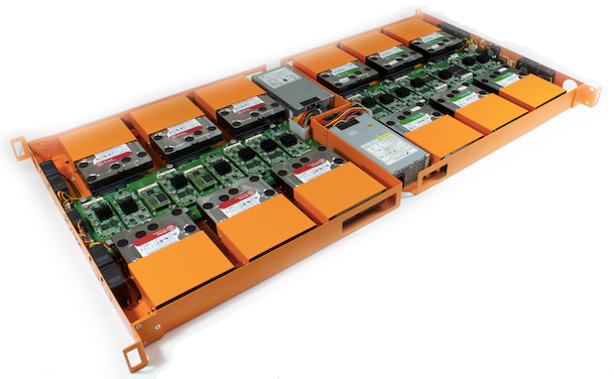
\includegraphics[scale=0.40]{img/CY7x2.png}\\
\caption{immagine1 \label{figura1.10} \cite{etichetta9}}
\end{figure}

\begin{figure}[htbp]
\centering
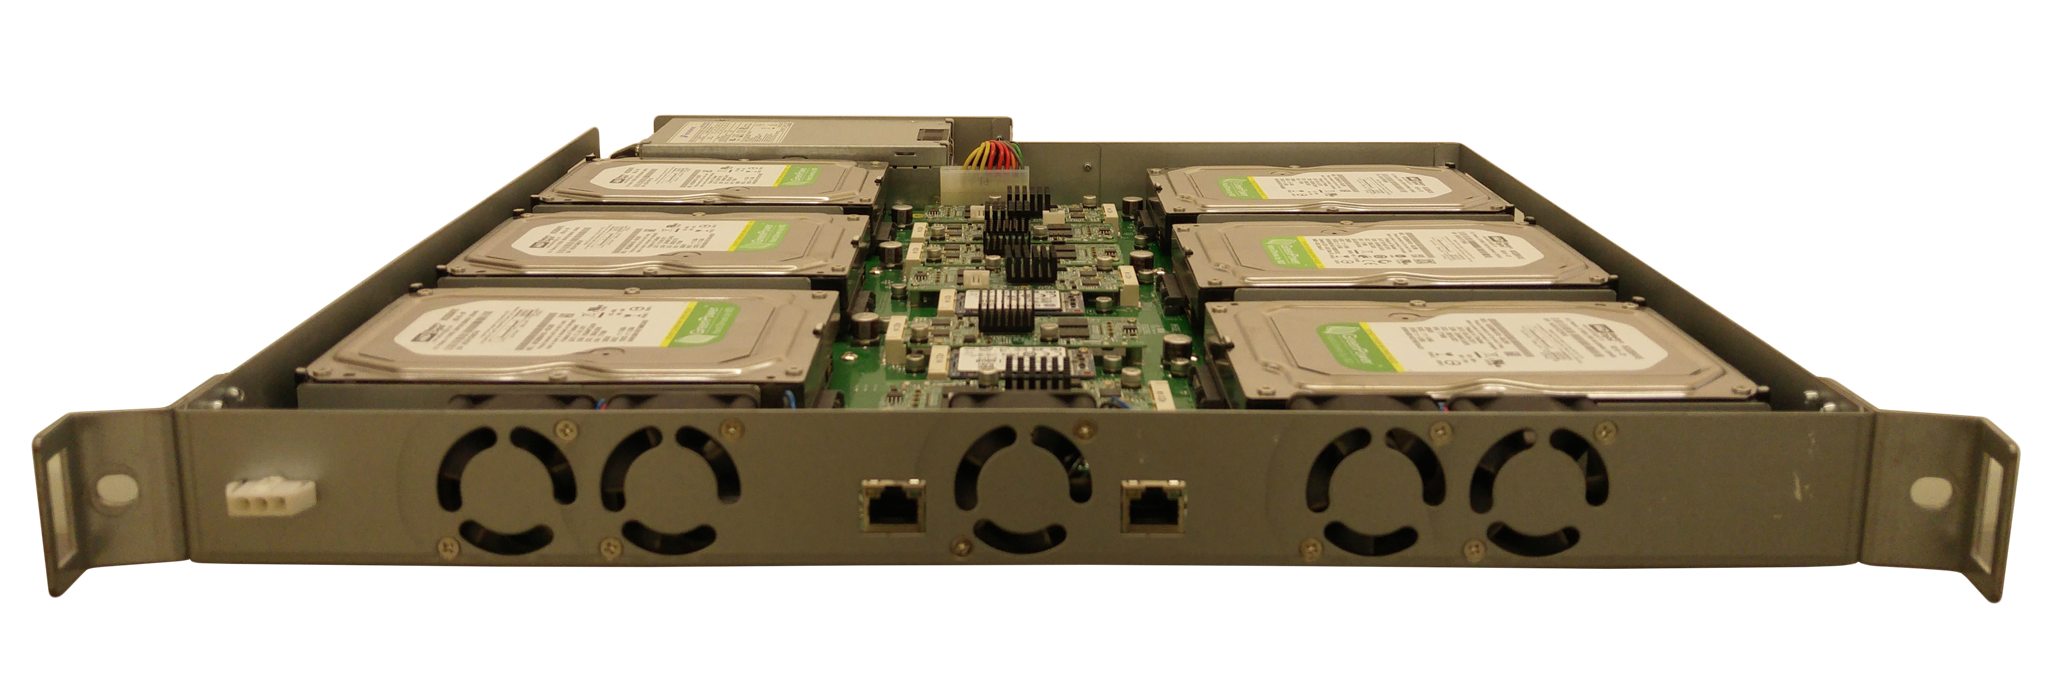
\includegraphics[scale=0.40]{img/CY7.png}\\
\caption{immagine2 \label{figura1.11} \cite{etichetta9}}
\end{figure}

\begin{figure}[htbp]
\centering
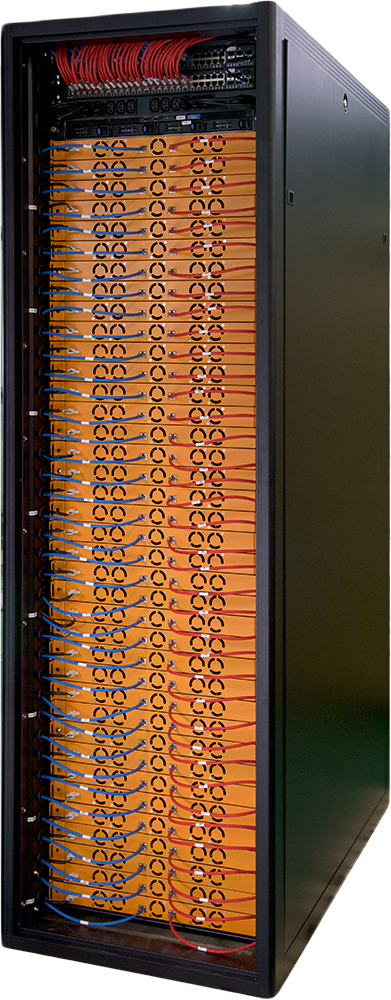
\includegraphics[scale=0.40]{img/rack.png}\\
\caption{rack \label{figura1.12} \cite{etichetta9}}
\end{figure}

\begin{figure}[htbp]
\centering
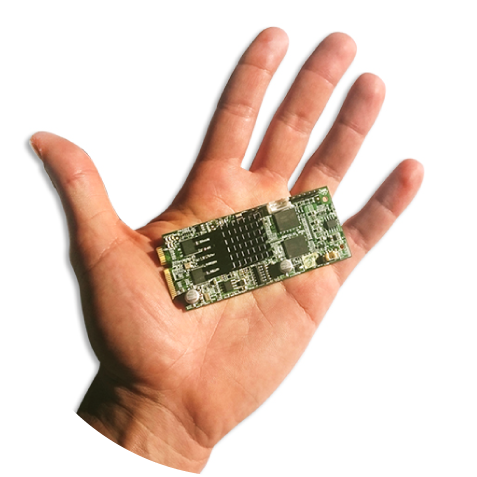
\includegraphics[scale=0.40]{img/Server.png}\\
\caption{server \label{figura1.13} \cite{etichetta9}}
\end{figure}